\section{Experiments \& Results}

The experiments were run in two Parts; Part 1- A classification task to classify a dataset containing 3 classes and 
Part 2- A classification task to classify the `MNIST' dataset.

\begin{figure}
    \centering
    \includegraphics[width=0.5\textwidth]{part_1_data.png}
    \caption[short]{Synthetic data}
    \label{fig: Synthetic data}
\end{figure}

\subsection{Part 1}

In this portion of the report, we delve into the experiments conducted and the
corresponding results obtained. Our primary objective was to ascertain the 
functionality of the developed program. A secondary goal involved investigating 
the effects of various activation functions: \textbf{Rectified Linear Unit (ReLU)}, 
\textbf{Sigmoid}, and \textbf{Hyperbolic Tangent (Tanh)} and the optimizers: 
\textbf{Stochastic Gradient Descent} and \textbf{Adaptive Momentum (Adam)}. 

\subsubsection{Data}
The dataset utilized for 
this analysis, depicted in Figure \ref{fig: Synthetic data}, was specifically 
crafted to be linearly separable. This design choice was made to simplify the 
verification process, as creating a discriminant function for a linearly 
separable dataset is relatively straightforward for a Neural Network employing 
non-linear activation functions. To this end, multiple architectures were 
explored, each incorporating one of the three aforementioned activation 
functions across all hidden layers. This approach facilitated a comparative 
analysis of the activation functions' performance within the framework of 
Multi-Layer Perceptron (MLP) models. 

\subsubsection{Model Architectures}
The `base model' was a 1 layered model that used the sigmoid activation function
across its hidden layers, shown in figure \ref{fig: NN 1l}. This architecture was 
designed with the minimum number of neurons required to create 3 functions in the
hidden layer which were supposed to have separated the 3 classes.

3 more `2 (hidden) layered models' (figure \ref{fig: NN 2l}) were created to compare firstly, the activation
functions and secondly, to the `base model'.


\begin{figure}
    \centering
    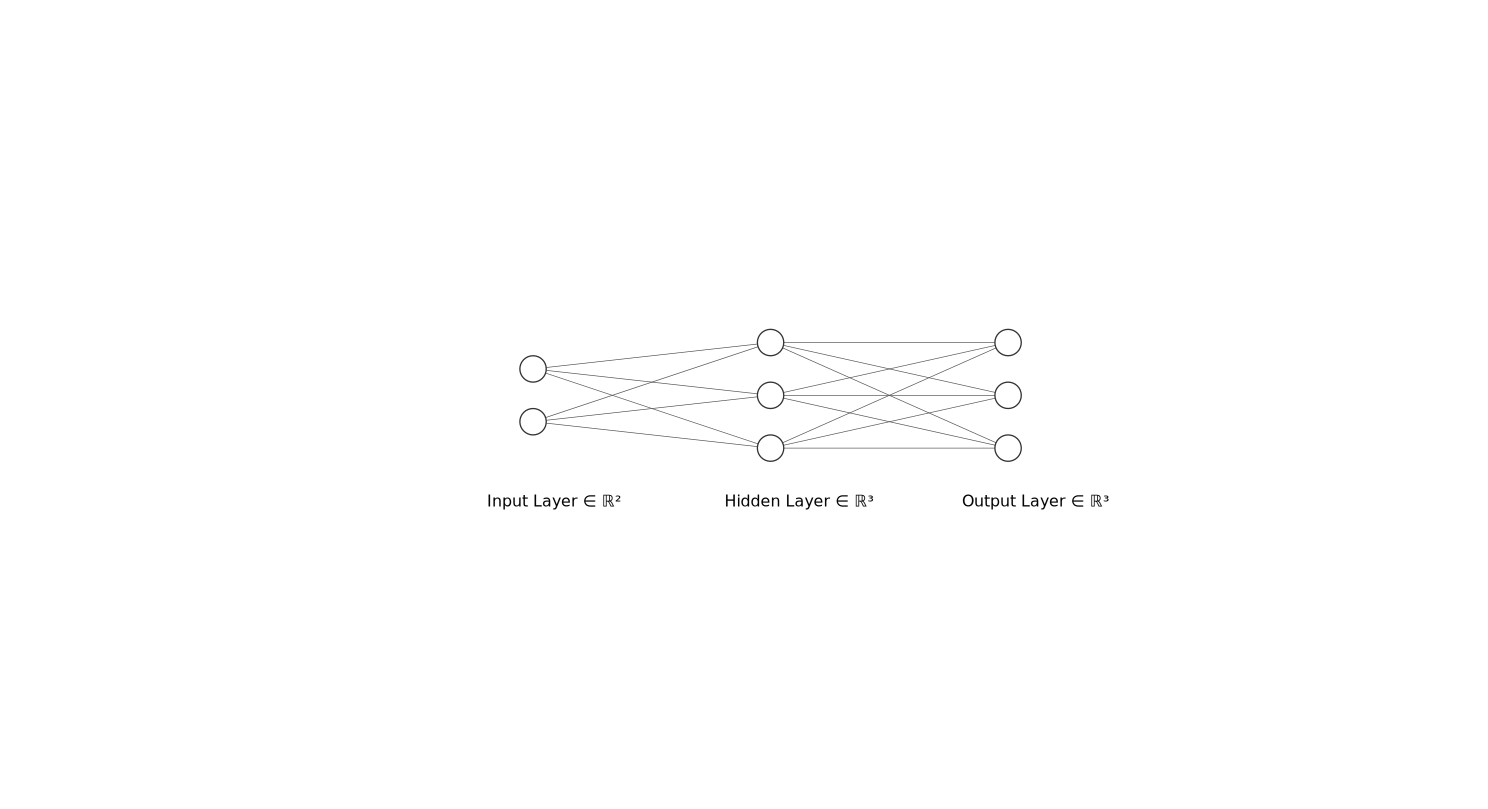
\includegraphics[width=0.8\textwidth]{sigmoid_1_layer.jpg}
    \caption{MLP with 1 hidden layer}
    \label{fig: NN 1l}
\end{figure}

\begin{figure}
    \centering
    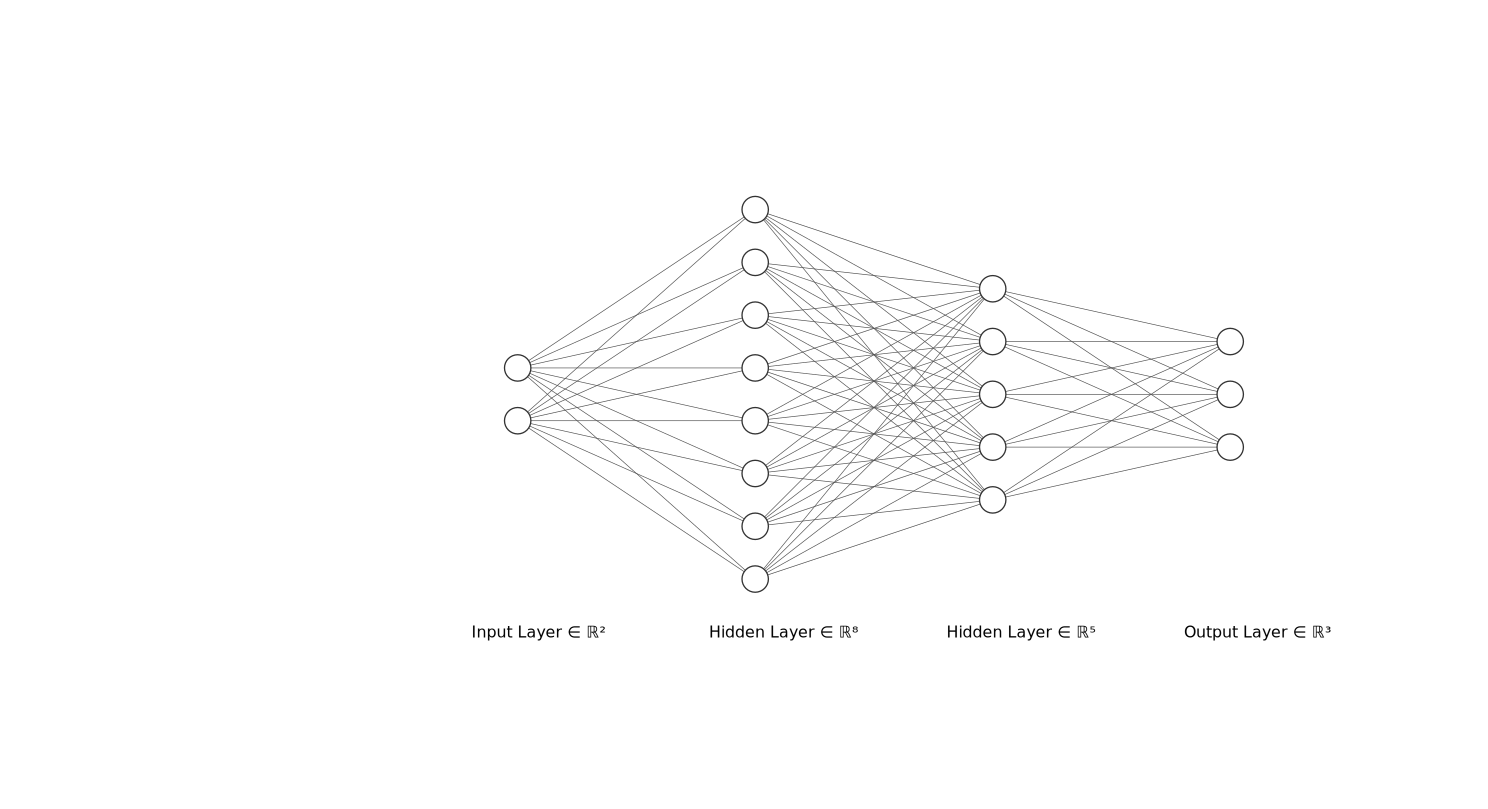
\includegraphics[width=0.8\textwidth]{sigmoid_2_layers.jpg}
    \caption{MLP with 2 hidden layers}
    \label{fig: NN 2l}
\end{figure}

\subsubsection{Training details}


\subsubsection{Results}

The accuracy-plot for all the architectures when using the Adam optimization algorithm is shown 
in figure \ref{fig: Adam results Part 1}

\begin{figure}
    \centering
    \includegraphics[width=1.0\textwidth]{./results/part_1_adam.png}
    \caption{Accuracy for Adam optimization}
    \label{fig: Adam results Part 1}
\end{figure}
